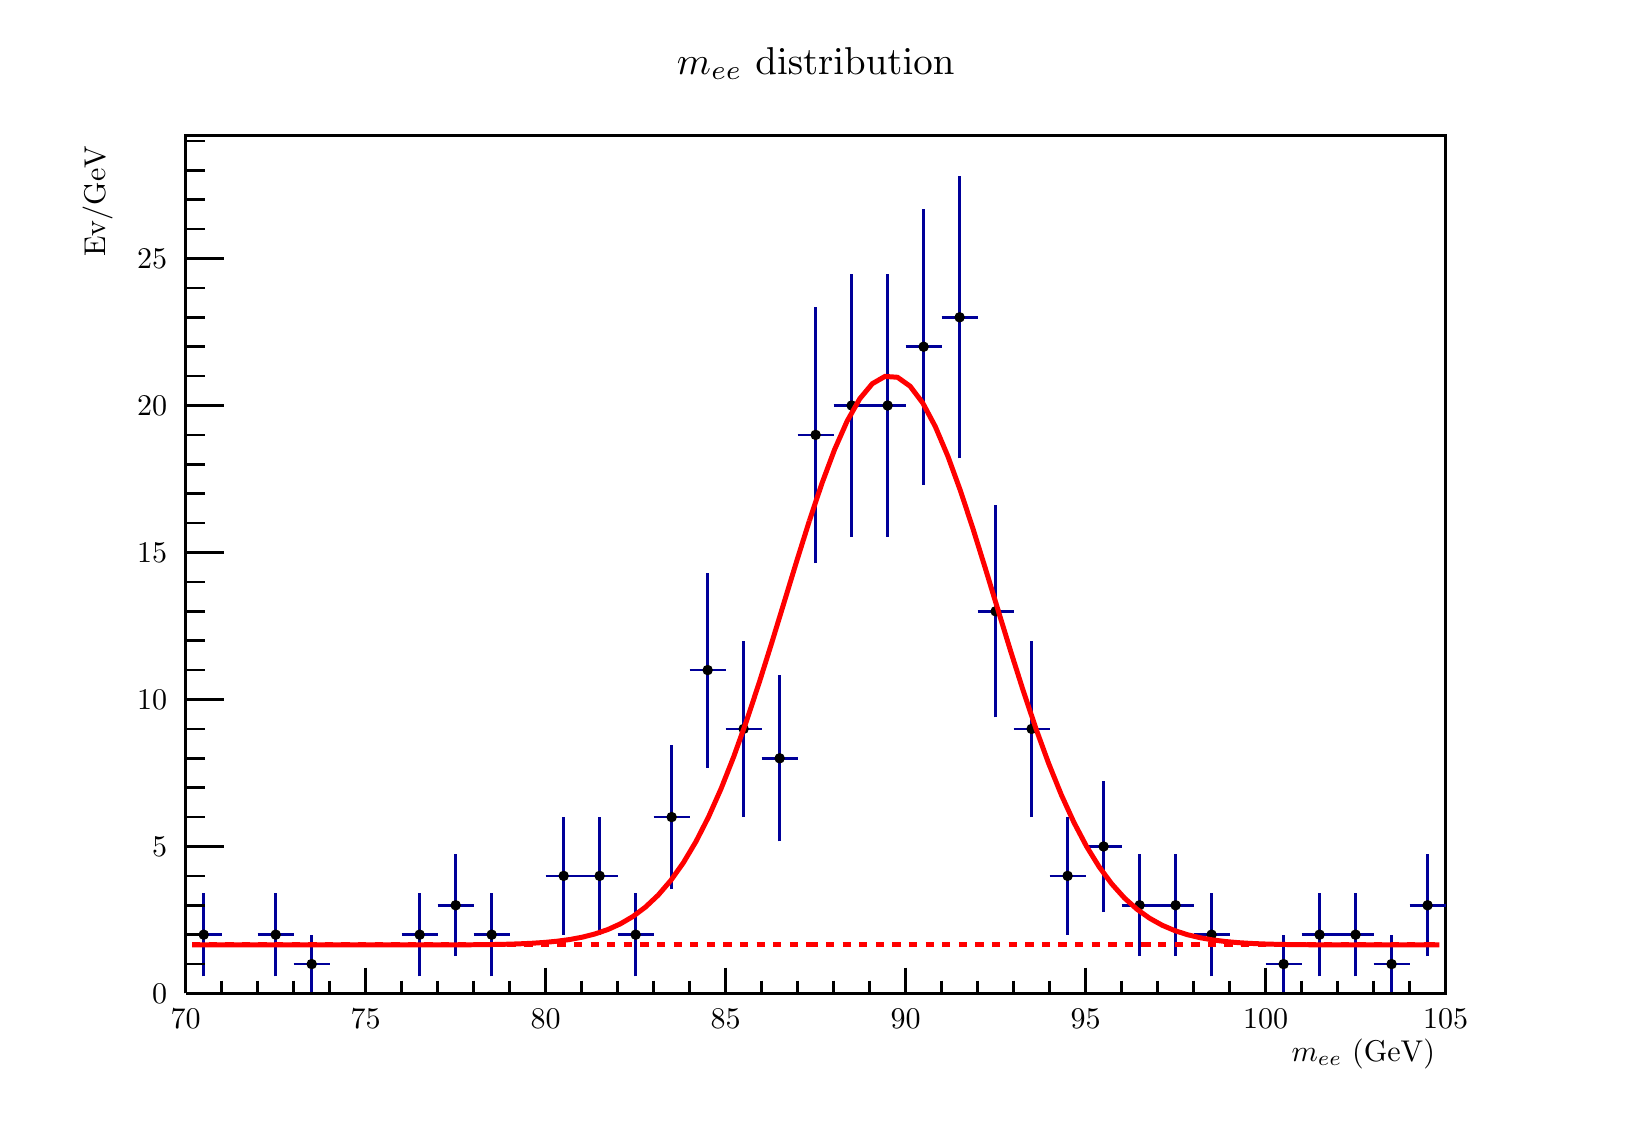
\begin{tikzpicture}
\pgfdeclareplotmark{cross} {
\pgfpathmoveto{\pgfpoint{-0.3\pgfplotmarksize}{\pgfplotmarksize}}
\pgfpathlineto{\pgfpoint{+0.3\pgfplotmarksize}{\pgfplotmarksize}}
\pgfpathlineto{\pgfpoint{+0.3\pgfplotmarksize}{0.3\pgfplotmarksize}}
\pgfpathlineto{\pgfpoint{+1\pgfplotmarksize}{0.3\pgfplotmarksize}}
\pgfpathlineto{\pgfpoint{+1\pgfplotmarksize}{-0.3\pgfplotmarksize}}
\pgfpathlineto{\pgfpoint{+0.3\pgfplotmarksize}{-0.3\pgfplotmarksize}}
\pgfpathlineto{\pgfpoint{+0.3\pgfplotmarksize}{-1.\pgfplotmarksize}}
\pgfpathlineto{\pgfpoint{-0.3\pgfplotmarksize}{-1.\pgfplotmarksize}}
\pgfpathlineto{\pgfpoint{-0.3\pgfplotmarksize}{-0.3\pgfplotmarksize}}
\pgfpathlineto{\pgfpoint{-1.\pgfplotmarksize}{-0.3\pgfplotmarksize}}
\pgfpathlineto{\pgfpoint{-1.\pgfplotmarksize}{0.3\pgfplotmarksize}}
\pgfpathlineto{\pgfpoint{-0.3\pgfplotmarksize}{0.3\pgfplotmarksize}}
\pgfpathclose
\pgfusepathqstroke
}
\pgfdeclareplotmark{cross*} {
\pgfpathmoveto{\pgfpoint{-0.3\pgfplotmarksize}{\pgfplotmarksize}}
\pgfpathlineto{\pgfpoint{+0.3\pgfplotmarksize}{\pgfplotmarksize}}
\pgfpathlineto{\pgfpoint{+0.3\pgfplotmarksize}{0.3\pgfplotmarksize}}
\pgfpathlineto{\pgfpoint{+1\pgfplotmarksize}{0.3\pgfplotmarksize}}
\pgfpathlineto{\pgfpoint{+1\pgfplotmarksize}{-0.3\pgfplotmarksize}}
\pgfpathlineto{\pgfpoint{+0.3\pgfplotmarksize}{-0.3\pgfplotmarksize}}
\pgfpathlineto{\pgfpoint{+0.3\pgfplotmarksize}{-1.\pgfplotmarksize}}
\pgfpathlineto{\pgfpoint{-0.3\pgfplotmarksize}{-1.\pgfplotmarksize}}
\pgfpathlineto{\pgfpoint{-0.3\pgfplotmarksize}{-0.3\pgfplotmarksize}}
\pgfpathlineto{\pgfpoint{-1.\pgfplotmarksize}{-0.3\pgfplotmarksize}}
\pgfpathlineto{\pgfpoint{-1.\pgfplotmarksize}{0.3\pgfplotmarksize}}
\pgfpathlineto{\pgfpoint{-0.3\pgfplotmarksize}{0.3\pgfplotmarksize}}
\pgfpathclose
\pgfusepathqfillstroke
}
\pgfdeclareplotmark{newstar} {
\pgfpathmoveto{\pgfqpoint{0pt}{\pgfplotmarksize}}
\pgfpathlineto{\pgfqpointpolar{44}{0.5\pgfplotmarksize}}
\pgfpathlineto{\pgfqpointpolar{18}{\pgfplotmarksize}}
\pgfpathlineto{\pgfqpointpolar{-20}{0.5\pgfplotmarksize}}
\pgfpathlineto{\pgfqpointpolar{-54}{\pgfplotmarksize}}
\pgfpathlineto{\pgfqpointpolar{-90}{0.5\pgfplotmarksize}}
\pgfpathlineto{\pgfqpointpolar{234}{\pgfplotmarksize}}
\pgfpathlineto{\pgfqpointpolar{198}{0.5\pgfplotmarksize}}
\pgfpathlineto{\pgfqpointpolar{162}{\pgfplotmarksize}}
\pgfpathlineto{\pgfqpointpolar{134}{0.5\pgfplotmarksize}}
\pgfpathclose
\pgfusepathqstroke
}
\pgfdeclareplotmark{newstar*} {
\pgfpathmoveto{\pgfqpoint{0pt}{\pgfplotmarksize}}
\pgfpathlineto{\pgfqpointpolar{44}{0.5\pgfplotmarksize}}
\pgfpathlineto{\pgfqpointpolar{18}{\pgfplotmarksize}}
\pgfpathlineto{\pgfqpointpolar{-20}{0.5\pgfplotmarksize}}
\pgfpathlineto{\pgfqpointpolar{-54}{\pgfplotmarksize}}
\pgfpathlineto{\pgfqpointpolar{-90}{0.5\pgfplotmarksize}}
\pgfpathlineto{\pgfqpointpolar{234}{\pgfplotmarksize}}
\pgfpathlineto{\pgfqpointpolar{198}{0.5\pgfplotmarksize}}
\pgfpathlineto{\pgfqpointpolar{162}{\pgfplotmarksize}}
\pgfpathlineto{\pgfqpointpolar{134}{0.5\pgfplotmarksize}}
\pgfpathclose
\pgfusepathqfillstroke
}
\definecolor{c}{rgb}{1,1,1};
\draw [color=c, fill=c] (0,0) rectangle (20,13.6207);
\draw [color=c, fill=c] (2,1.36207) rectangle (18,12.2586);
\definecolor{c}{rgb}{0,0,0};
\draw [c,line width=0.9] (2,1.36207) -- (2,12.2586) -- (18,12.2586) -- (18,1.36207) -- (2,1.36207);
\definecolor{c}{rgb}{1,1,1};
\draw [color=c, fill=c] (2,1.36207) rectangle (18,12.2586);
\definecolor{c}{rgb}{0,0,0};
\draw [c,line width=0.9] (2,1.36207) -- (2,12.2586) -- (18,12.2586) -- (18,1.36207) -- (2,1.36207);
\definecolor{c}{rgb}{0,0,0.6};
\draw [c,line width=0.9] (2.22857,1.58077) -- (2.22857,2.0513);
\draw [c,line width=0.9] (2.22857,2.16625) -- (2.22857,2.63678);
\draw [c,line width=0.9] (2,2.10878) -- (2.1711,2.10878);
\draw [c,line width=0.9] (2.28604,2.10878) -- (2.45714,2.10878);
\definecolor{c}{rgb}{0,0,0};
\foreach \P in {(2.22857,2.10878)}{\draw[mark options={color=c,fill=c},mark size=1.681682pt,mark=*] plot coordinates {\P};}
\definecolor{c}{rgb}{0,0,0.6};
\draw [c,line width=0.9] (3.14286,1.58077) -- (3.14286,2.0513);
\draw [c,line width=0.9] (3.14286,2.16625) -- (3.14286,2.63678);
\draw [c,line width=0.9] (2.91429,2.10878) -- (3.08539,2.10878);
\draw [c,line width=0.9] (3.20033,2.10878) -- (3.37143,2.10878);
\definecolor{c}{rgb}{0,0,0};
\foreach \P in {(3.14286,2.10878)}{\draw[mark options={color=c,fill=c},mark size=1.681682pt,mark=*] plot coordinates {\P};}
\definecolor{c}{rgb}{0,0,0.6};
\draw [c,line width=0.9] (3.6,1.36207) -- (3.6,1.67795);
\draw [c,line width=0.9] (3.6,1.79289) -- (3.6,2.10878);
\draw [c,line width=0.9] (3.37143,1.73542) -- (3.54253,1.73542);
\draw [c,line width=0.9] (3.65747,1.73542) -- (3.82857,1.73542);
\definecolor{c}{rgb}{0,0,0};
\foreach \P in {(3.6,1.73542)}{\draw[mark options={color=c,fill=c},mark size=1.681682pt,mark=*] plot coordinates {\P};}
\definecolor{c}{rgb}{0,0,0.6};
\draw [c,line width=0.9] (4.97143,1.58077) -- (4.97143,2.0513);
\draw [c,line width=0.9] (4.97143,2.16625) -- (4.97143,2.63678);
\draw [c,line width=0.9] (4.74286,2.10878) -- (4.91396,2.10878);
\draw [c,line width=0.9] (5.0289,2.10878) -- (5.2,2.10878);
\definecolor{c}{rgb}{0,0,0};
\foreach \P in {(4.97143,2.10878)}{\draw[mark options={color=c,fill=c},mark size=1.681682pt,mark=*] plot coordinates {\P};}
\definecolor{c}{rgb}{0,0,0.6};
\draw [c,line width=0.9] (5.42857,1.83546) -- (5.42857,2.42466);
\draw [c,line width=0.9] (5.42857,2.5396) -- (5.42857,3.1288);
\draw [c,line width=0.9] (5.2,2.48213) -- (5.3711,2.48213);
\draw [c,line width=0.9] (5.48604,2.48213) -- (5.65714,2.48213);
\definecolor{c}{rgb}{0,0,0};
\foreach \P in {(5.42857,2.48213)}{\draw[mark options={color=c,fill=c},mark size=1.681682pt,mark=*] plot coordinates {\P};}
\definecolor{c}{rgb}{0,0,0.6};
\draw [c,line width=0.9] (5.88571,1.58077) -- (5.88571,2.0513);
\draw [c,line width=0.9] (5.88571,2.16625) -- (5.88571,2.63678);
\draw [c,line width=0.9] (5.65714,2.10878) -- (5.82824,2.10878);
\draw [c,line width=0.9] (5.94319,2.10878) -- (6.11429,2.10878);
\definecolor{c}{rgb}{0,0,0};
\foreach \P in {(5.88571,2.10878)}{\draw[mark options={color=c,fill=c},mark size=1.681682pt,mark=*] plot coordinates {\P};}
\definecolor{c}{rgb}{0,0,0.6};
\draw [c,line width=0.9] (6.8,2.10878) -- (6.8,2.79801);
\draw [c,line width=0.9] (6.8,2.91295) -- (6.8,3.60219);
\draw [c,line width=0.9] (6.57143,2.85548) -- (6.74253,2.85548);
\draw [c,line width=0.9] (6.85747,2.85548) -- (7.02857,2.85548);
\definecolor{c}{rgb}{0,0,0};
\foreach \P in {(6.8,2.85548)}{\draw[mark options={color=c,fill=c},mark size=1.681682pt,mark=*] plot coordinates {\P};}
\definecolor{c}{rgb}{0,0,0.6};
\draw [c,line width=0.9] (7.25714,2.10878) -- (7.25714,2.79801);
\draw [c,line width=0.9] (7.25714,2.91295) -- (7.25714,3.60219);
\draw [c,line width=0.9] (7.02857,2.85548) -- (7.19967,2.85548);
\draw [c,line width=0.9] (7.31461,2.85548) -- (7.48571,2.85548);
\definecolor{c}{rgb}{0,0,0};
\foreach \P in {(7.25714,2.85548)}{\draw[mark options={color=c,fill=c},mark size=1.681682pt,mark=*] plot coordinates {\P};}
\definecolor{c}{rgb}{0,0,0.6};
\draw [c,line width=0.9] (7.71429,1.58077) -- (7.71429,2.0513);
\draw [c,line width=0.9] (7.71429,2.16625) -- (7.71429,2.63678);
\draw [c,line width=0.9] (7.48571,2.10878) -- (7.65681,2.10878);
\draw [c,line width=0.9] (7.77176,2.10878) -- (7.94286,2.10878);
\definecolor{c}{rgb}{0,0,0};
\foreach \P in {(7.71429,2.10878)}{\draw[mark options={color=c,fill=c},mark size=1.681682pt,mark=*] plot coordinates {\P};}
\definecolor{c}{rgb}{0,0,0.6};
\draw [c,line width=0.9] (8.17143,2.68766) -- (8.17143,3.54472);
\draw [c,line width=0.9] (8.17143,3.65966) -- (8.17143,4.51671);
\draw [c,line width=0.9] (7.94286,3.60219) -- (8.11396,3.60219);
\draw [c,line width=0.9] (8.2289,3.60219) -- (8.4,3.60219);
\definecolor{c}{rgb}{0,0,0};
\foreach \P in {(8.17143,3.60219)}{\draw[mark options={color=c,fill=c},mark size=1.681682pt,mark=*] plot coordinates {\P};}
\definecolor{c}{rgb}{0,0,0.6};
\draw [c,line width=0.9] (8.62857,4.23068) -- (8.62857,5.41149);
\draw [c,line width=0.9] (8.62857,5.52643) -- (8.62857,6.70723);
\draw [c,line width=0.9] (8.4,5.46896) -- (8.5711,5.46896);
\draw [c,line width=0.9] (8.68604,5.46896) -- (8.85714,5.46896);
\definecolor{c}{rgb}{0,0,0};
\foreach \P in {(8.62857,5.46896)}{\draw[mark options={color=c,fill=c},mark size=1.681682pt,mark=*] plot coordinates {\P};}
\definecolor{c}{rgb}{0,0,0.6};
\draw [c,line width=0.9] (9.08571,3.60219) -- (9.08571,4.66478);
\draw [c,line width=0.9] (9.08571,4.77972) -- (9.08571,5.84231);
\draw [c,line width=0.9] (8.85714,4.72225) -- (9.02824,4.72225);
\draw [c,line width=0.9] (9.14319,4.72225) -- (9.31429,4.72225);
\definecolor{c}{rgb}{0,0,0};
\foreach \P in {(9.08571,4.72225)}{\draw[mark options={color=c,fill=c},mark size=1.681682pt,mark=*] plot coordinates {\P};}
\definecolor{c}{rgb}{0,0,0.6};
\draw [c,line width=0.9] (9.54286,3.29289) -- (9.54286,4.29142);
\draw [c,line width=0.9] (9.54286,4.40637) -- (9.54286,5.4049);
\draw [c,line width=0.9] (9.31429,4.3489) -- (9.48539,4.3489);
\draw [c,line width=0.9] (9.60033,4.3489) -- (9.77143,4.3489);
\definecolor{c}{rgb}{0,0,0};
\foreach \P in {(9.54286,4.3489)}{\draw[mark options={color=c,fill=c},mark size=1.681682pt,mark=*] plot coordinates {\P};}
\definecolor{c}{rgb}{0,0,0.6};
\draw [c,line width=0.9] (10,6.82837) -- (10,8.39831);
\draw [c,line width=0.9] (10,8.51326) -- (10,10.0832);
\draw [c,line width=0.9] (9.77143,8.45578) -- (9.94253,8.45578);
\draw [c,line width=0.9] (10.0575,8.45578) -- (10.2286,8.45578);
\definecolor{c}{rgb}{0,0,0};
\foreach \P in {(10,8.45578)}{\draw[mark options={color=c,fill=c},mark size=1.681682pt,mark=*] plot coordinates {\P};}
\definecolor{c}{rgb}{0,0,0.6};
\draw [c,line width=0.9] (10.4571,7.15945) -- (10.4571,8.77167);
\draw [c,line width=0.9] (10.4571,8.88661) -- (10.4571,10.4988);
\draw [c,line width=0.9] (10.2286,8.82914) -- (10.3997,8.82914);
\draw [c,line width=0.9] (10.5146,8.82914) -- (10.6857,8.82914);
\definecolor{c}{rgb}{0,0,0};
\foreach \P in {(10.4571,8.82914)}{\draw[mark options={color=c,fill=c},mark size=1.681682pt,mark=*] plot coordinates {\P};}
\definecolor{c}{rgb}{0,0,0.6};
\draw [c,line width=0.9] (10.9143,7.15945) -- (10.9143,8.77167);
\draw [c,line width=0.9] (10.9143,8.88661) -- (10.9143,10.4988);
\draw [c,line width=0.9] (10.6857,8.82914) -- (10.8568,8.82914);
\draw [c,line width=0.9] (10.9718,8.82914) -- (11.1429,8.82914);
\definecolor{c}{rgb}{0,0,0};
\foreach \P in {(10.9143,8.82914)}{\draw[mark options={color=c,fill=c},mark size=1.681682pt,mark=*] plot coordinates {\P};}
\definecolor{c}{rgb}{0,0,0.6};
\draw [c,line width=0.9] (11.3714,7.82466) -- (11.3714,9.51837);
\draw [c,line width=0.9] (11.3714,9.63332) -- (11.3714,11.327);
\draw [c,line width=0.9] (11.1429,9.57584) -- (11.314,9.57584);
\draw [c,line width=0.9] (11.4289,9.57584) -- (11.6,9.57584);
\definecolor{c}{rgb}{0,0,0};
\foreach \P in {(11.3714,9.57584)}{\draw[mark options={color=c,fill=c},mark size=1.681682pt,mark=*] plot coordinates {\P};}
\definecolor{c}{rgb}{0,0,0.6};
\draw [c,line width=0.9] (11.8286,8.15866) -- (11.8286,9.89173);
\draw [c,line width=0.9] (11.8286,10.0067) -- (11.8286,11.7397);
\draw [c,line width=0.9] (11.6,9.9492) -- (11.7711,9.9492);
\draw [c,line width=0.9] (11.886,9.9492) -- (12.0571,9.9492);
\definecolor{c}{rgb}{0,0,0};
\foreach \P in {(11.8286,9.9492)}{\draw[mark options={color=c,fill=c},mark size=1.681682pt,mark=*] plot coordinates {\P};}
\definecolor{c}{rgb}{0,0,0.6};
\draw [c,line width=0.9] (12.2857,4.86952) -- (12.2857,6.15819);
\draw [c,line width=0.9] (12.2857,6.27313) -- (12.2857,7.56181);
\draw [c,line width=0.9] (12.0571,6.21566) -- (12.2282,6.21566);
\draw [c,line width=0.9] (12.3432,6.21566) -- (12.5143,6.21566);
\definecolor{c}{rgb}{0,0,0};
\foreach \P in {(12.2857,6.21566)}{\draw[mark options={color=c,fill=c},mark size=1.681682pt,mark=*] plot coordinates {\P};}
\definecolor{c}{rgb}{0,0,0.6};
\draw [c,line width=0.9] (12.7429,3.60219) -- (12.7429,4.66478);
\draw [c,line width=0.9] (12.7429,4.77972) -- (12.7429,5.84231);
\draw [c,line width=0.9] (12.5143,4.72225) -- (12.6854,4.72225);
\draw [c,line width=0.9] (12.8003,4.72225) -- (12.9714,4.72225);
\definecolor{c}{rgb}{0,0,0};
\foreach \P in {(12.7429,4.72225)}{\draw[mark options={color=c,fill=c},mark size=1.681682pt,mark=*] plot coordinates {\P};}
\definecolor{c}{rgb}{0,0,0.6};
\draw [c,line width=0.9] (13.2,2.10878) -- (13.2,2.79801);
\draw [c,line width=0.9] (13.2,2.91295) -- (13.2,3.60219);
\draw [c,line width=0.9] (12.9714,2.85548) -- (13.1425,2.85548);
\draw [c,line width=0.9] (13.2575,2.85548) -- (13.4286,2.85548);
\definecolor{c}{rgb}{0,0,0};
\foreach \P in {(13.2,2.85548)}{\draw[mark options={color=c,fill=c},mark size=1.681682pt,mark=*] plot coordinates {\P};}
\definecolor{c}{rgb}{0,0,0.6};
\draw [c,line width=0.9] (13.6571,2.39399) -- (13.6571,3.17136);
\draw [c,line width=0.9] (13.6571,3.28631) -- (13.6571,4.06368);
\draw [c,line width=0.9] (13.4286,3.22884) -- (13.5997,3.22884);
\draw [c,line width=0.9] (13.7146,3.22884) -- (13.8857,3.22884);
\definecolor{c}{rgb}{0,0,0};
\foreach \P in {(13.6571,3.22884)}{\draw[mark options={color=c,fill=c},mark size=1.681682pt,mark=*] plot coordinates {\P};}
\definecolor{c}{rgb}{0,0,0.6};
\draw [c,line width=0.9] (14.1143,1.83546) -- (14.1143,2.42466);
\draw [c,line width=0.9] (14.1143,2.5396) -- (14.1143,3.1288);
\draw [c,line width=0.9] (13.8857,2.48213) -- (14.0568,2.48213);
\draw [c,line width=0.9] (14.1718,2.48213) -- (14.3429,2.48213);
\definecolor{c}{rgb}{0,0,0};
\foreach \P in {(14.1143,2.48213)}{\draw[mark options={color=c,fill=c},mark size=1.681682pt,mark=*] plot coordinates {\P};}
\definecolor{c}{rgb}{0,0,0.6};
\draw [c,line width=0.9] (14.5714,1.83546) -- (14.5714,2.42466);
\draw [c,line width=0.9] (14.5714,2.5396) -- (14.5714,3.1288);
\draw [c,line width=0.9] (14.3429,2.48213) -- (14.514,2.48213);
\draw [c,line width=0.9] (14.6289,2.48213) -- (14.8,2.48213);
\definecolor{c}{rgb}{0,0,0};
\foreach \P in {(14.5714,2.48213)}{\draw[mark options={color=c,fill=c},mark size=1.681682pt,mark=*] plot coordinates {\P};}
\definecolor{c}{rgb}{0,0,0.6};
\draw [c,line width=0.9] (15.0286,1.58077) -- (15.0286,2.0513);
\draw [c,line width=0.9] (15.0286,2.16625) -- (15.0286,2.63678);
\draw [c,line width=0.9] (14.8,2.10878) -- (14.9711,2.10878);
\draw [c,line width=0.9] (15.086,2.10878) -- (15.2571,2.10878);
\definecolor{c}{rgb}{0,0,0};
\foreach \P in {(15.0286,2.10878)}{\draw[mark options={color=c,fill=c},mark size=1.681682pt,mark=*] plot coordinates {\P};}
\definecolor{c}{rgb}{0,0,0.6};
\draw [c,line width=0.9] (15.9429,1.36207) -- (15.9429,1.67795);
\draw [c,line width=0.9] (15.9429,1.79289) -- (15.9429,2.10878);
\draw [c,line width=0.9] (15.7143,1.73542) -- (15.8854,1.73542);
\draw [c,line width=0.9] (16.0003,1.73542) -- (16.1714,1.73542);
\definecolor{c}{rgb}{0,0,0};
\foreach \P in {(15.9429,1.73542)}{\draw[mark options={color=c,fill=c},mark size=1.681682pt,mark=*] plot coordinates {\P};}
\definecolor{c}{rgb}{0,0,0.6};
\draw [c,line width=0.9] (16.4,1.58077) -- (16.4,2.0513);
\draw [c,line width=0.9] (16.4,2.16625) -- (16.4,2.63678);
\draw [c,line width=0.9] (16.1714,2.10878) -- (16.3425,2.10878);
\draw [c,line width=0.9] (16.4575,2.10878) -- (16.6286,2.10878);
\definecolor{c}{rgb}{0,0,0};
\foreach \P in {(16.4,2.10878)}{\draw[mark options={color=c,fill=c},mark size=1.681682pt,mark=*] plot coordinates {\P};}
\definecolor{c}{rgb}{0,0,0.6};
\draw [c,line width=0.9] (16.8571,1.58077) -- (16.8571,2.0513);
\draw [c,line width=0.9] (16.8571,2.16625) -- (16.8571,2.63678);
\draw [c,line width=0.9] (16.6286,2.10878) -- (16.7997,2.10878);
\draw [c,line width=0.9] (16.9146,2.10878) -- (17.0857,2.10878);
\definecolor{c}{rgb}{0,0,0};
\foreach \P in {(16.8571,2.10878)}{\draw[mark options={color=c,fill=c},mark size=1.681682pt,mark=*] plot coordinates {\P};}
\definecolor{c}{rgb}{0,0,0.6};
\draw [c,line width=0.9] (17.3143,1.36207) -- (17.3143,1.67795);
\draw [c,line width=0.9] (17.3143,1.79289) -- (17.3143,2.10878);
\draw [c,line width=0.9] (17.0857,1.73542) -- (17.2568,1.73542);
\draw [c,line width=0.9] (17.3718,1.73542) -- (17.5429,1.73542);
\definecolor{c}{rgb}{0,0,0};
\foreach \P in {(17.3143,1.73542)}{\draw[mark options={color=c,fill=c},mark size=1.681682pt,mark=*] plot coordinates {\P};}
\definecolor{c}{rgb}{0,0,0.6};
\draw [c,line width=0.9] (17.7714,1.83546) -- (17.7714,2.42466);
\draw [c,line width=0.9] (17.7714,2.5396) -- (17.7714,3.1288);
\draw [c,line width=0.9] (17.5429,2.48213) -- (17.714,2.48213);
\draw [c,line width=0.9] (17.8289,2.48213) -- (18,2.48213);
\definecolor{c}{rgb}{0,0,0};
\foreach \P in {(17.7714,2.48213)}{\draw[mark options={color=c,fill=c},mark size=1.681682pt,mark=*] plot coordinates {\P};}
\definecolor{c}{rgb}{1,0,0};
\draw [c,line width=1.8] (2.08,1.9781) -- (2.24,1.9781) -- (2.4,1.9781) -- (2.56,1.9781) -- (2.72,1.9781) -- (2.88,1.9781) -- (3.04,1.9781) -- (3.2,1.9781) -- (3.36,1.9781) -- (3.52,1.9781) -- (3.68,1.9781) -- (3.84,1.97811) -- (4,1.97811) --
 (4.16,1.97812) -- (4.32,1.97813) -- (4.48,1.97816) -- (4.64,1.9782) -- (4.8,1.97828) -- (4.96,1.97841) -- (5.12,1.97862) -- (5.28,1.97898) -- (5.44,1.97955) -- (5.6,1.98046) -- (5.76,1.98189) -- (5.92,1.9841) -- (6.08,1.98745) -- (6.24,1.99248) --
 (6.4,1.9999) -- (6.56,2.01067) -- (6.72,2.02607) -- (6.88,2.04775) -- (7.04,2.07777) -- (7.2,2.11869) -- (7.36,2.17359) -- (7.52,2.24603) -- (7.68,2.34006) -- (7.84,2.46011) -- (8,2.6108) -- (8.16,2.79673) -- (8.32,3.02216) -- (8.48,3.29063) --
 (8.64,3.60455) -- (8.8,3.96475) -- (8.96,4.37003) -- (9.12,4.81682) -- (9.28,5.29891) -- (9.44,5.80734) -- (9.6,6.33051) -- (9.76,6.85443) -- (9.92,7.36334);
\draw [c,line width=1.8] (9.92,7.36334) -- (10.08,7.84034) -- (10.24,8.26838) -- (10.4,8.6312) -- (10.56,8.91436) -- (10.72,9.10621) -- (10.88,9.19865) -- (11.04,9.18775) -- (11.2,9.07396) -- (11.36,8.86214) -- (11.52,8.56119) -- (11.68,8.1834) --
 (11.84,7.74369) -- (12,7.25856) -- (12.16,6.74513) -- (12.32,6.2201) -- (12.48,5.69895) -- (12.64,5.19516) -- (12.8,4.71983) -- (12.96,4.28133) -- (13.12,3.88531) -- (13.28,3.53481) -- (13.44,3.23055) -- (13.6,2.97136) -- (13.76,2.75455) --
 (13.92,2.57639) -- (14.08,2.43252) -- (14.24,2.31831) -- (14.4,2.22917) -- (14.56,2.16073) -- (14.72,2.10905) -- (14.88,2.07066) -- (15.04,2.04258) -- (15.2,2.02238) -- (15.36,2.00807) -- (15.52,1.9981) -- (15.68,1.99125) -- (15.84,1.98663) --
 (16,1.98355) -- (16.16,1.98153) -- (16.32,1.98023) -- (16.48,1.97941) -- (16.64,1.97889) -- (16.8,1.97857) -- (16.96,1.97838) -- (17.12,1.97826) -- (17.28,1.97819) -- (17.44,1.97815) -- (17.6,1.97813) -- (17.76,1.97812);
\draw [c,line width=1.8] (17.76,1.97812) -- (17.92,1.97811);
\definecolor{c}{rgb}{0,0,0};
\draw [c,line width=0.9] (2,1.36207) -- (18,1.36207);
\draw [anchor= east] (18,0.599311) node[scale=1.08496, color=c, rotate=0]{$m_{ee} \mbox{ (GeV)}$};
\draw [c,line width=0.9] (2,1.68897) -- (2,1.36207);
\draw [c,line width=0.9] (2.45714,1.52552) -- (2.45714,1.36207);
\draw [c,line width=0.9] (2.91429,1.52552) -- (2.91429,1.36207);
\draw [c,line width=0.9] (3.37143,1.52552) -- (3.37143,1.36207);
\draw [c,line width=0.9] (3.82857,1.52552) -- (3.82857,1.36207);
\draw [c,line width=0.9] (4.28571,1.68897) -- (4.28571,1.36207);
\draw [c,line width=0.9] (4.74286,1.52552) -- (4.74286,1.36207);
\draw [c,line width=0.9] (5.2,1.52552) -- (5.2,1.36207);
\draw [c,line width=0.9] (5.65714,1.52552) -- (5.65714,1.36207);
\draw [c,line width=0.9] (6.11429,1.52552) -- (6.11429,1.36207);
\draw [c,line width=0.9] (6.57143,1.68897) -- (6.57143,1.36207);
\draw [c,line width=0.9] (7.02857,1.52552) -- (7.02857,1.36207);
\draw [c,line width=0.9] (7.48571,1.52552) -- (7.48571,1.36207);
\draw [c,line width=0.9] (7.94286,1.52552) -- (7.94286,1.36207);
\draw [c,line width=0.9] (8.4,1.52552) -- (8.4,1.36207);
\draw [c,line width=0.9] (8.85714,1.68897) -- (8.85714,1.36207);
\draw [c,line width=0.9] (9.31429,1.52552) -- (9.31429,1.36207);
\draw [c,line width=0.9] (9.77143,1.52552) -- (9.77143,1.36207);
\draw [c,line width=0.9] (10.2286,1.52552) -- (10.2286,1.36207);
\draw [c,line width=0.9] (10.6857,1.52552) -- (10.6857,1.36207);
\draw [c,line width=0.9] (11.1429,1.68897) -- (11.1429,1.36207);
\draw [c,line width=0.9] (11.6,1.52552) -- (11.6,1.36207);
\draw [c,line width=0.9] (12.0571,1.52552) -- (12.0571,1.36207);
\draw [c,line width=0.9] (12.5143,1.52552) -- (12.5143,1.36207);
\draw [c,line width=0.9] (12.9714,1.52552) -- (12.9714,1.36207);
\draw [c,line width=0.9] (13.4286,1.68897) -- (13.4286,1.36207);
\draw [c,line width=0.9] (13.8857,1.52552) -- (13.8857,1.36207);
\draw [c,line width=0.9] (14.3429,1.52552) -- (14.3429,1.36207);
\draw [c,line width=0.9] (14.8,1.52552) -- (14.8,1.36207);
\draw [c,line width=0.9] (15.2571,1.52552) -- (15.2571,1.36207);
\draw [c,line width=0.9] (15.7143,1.68897) -- (15.7143,1.36207);
\draw [c,line width=0.9] (16.1714,1.52552) -- (16.1714,1.36207);
\draw [c,line width=0.9] (16.6286,1.52552) -- (16.6286,1.36207);
\draw [c,line width=0.9] (17.0857,1.52552) -- (17.0857,1.36207);
\draw [c,line width=0.9] (17.5429,1.52552) -- (17.5429,1.36207);
\draw [c,line width=0.9] (18,1.68897) -- (18,1.36207);
\draw [anchor=base] (2,0.912586) node[scale=1.08496, color=c, rotate=0]{70};
\draw [anchor=base] (4.28571,0.912586) node[scale=1.08496, color=c, rotate=0]{75};
\draw [anchor=base] (6.57143,0.912586) node[scale=1.08496, color=c, rotate=0]{80};
\draw [anchor=base] (8.85714,0.912586) node[scale=1.08496, color=c, rotate=0]{85};
\draw [anchor=base] (11.1429,0.912586) node[scale=1.08496, color=c, rotate=0]{90};
\draw [anchor=base] (13.4286,0.912586) node[scale=1.08496, color=c, rotate=0]{95};
\draw [anchor=base] (15.7143,0.912586) node[scale=1.08496, color=c, rotate=0]{100};
\draw [anchor=base] (18,0.912586) node[scale=1.08496, color=c, rotate=0]{105};
\draw [c,line width=0.9] (2,1.36207) -- (2,12.2586);
\draw [anchor= east] (0.88,12.2586) node[scale=1.08496, color=c, rotate=90]{$\mbox{Ev/GeV}$};
\draw [c,line width=0.9] (2.48,1.36207) -- (2,1.36207);
\draw [c,line width=0.9] (2.24,1.73542) -- (2,1.73542);
\draw [c,line width=0.9] (2.24,2.10878) -- (2,2.10878);
\draw [c,line width=0.9] (2.24,2.48213) -- (2,2.48213);
\draw [c,line width=0.9] (2.24,2.85548) -- (2,2.85548);
\draw [c,line width=0.9] (2.48,3.22884) -- (2,3.22884);
\draw [c,line width=0.9] (2.24,3.60219) -- (2,3.60219);
\draw [c,line width=0.9] (2.24,3.97554) -- (2,3.97554);
\draw [c,line width=0.9] (2.24,4.3489) -- (2,4.3489);
\draw [c,line width=0.9] (2.24,4.72225) -- (2,4.72225);
\draw [c,line width=0.9] (2.48,5.0956) -- (2,5.0956);
\draw [c,line width=0.9] (2.24,5.46896) -- (2,5.46896);
\draw [c,line width=0.9] (2.24,5.84231) -- (2,5.84231);
\draw [c,line width=0.9] (2.24,6.21566) -- (2,6.21566);
\draw [c,line width=0.9] (2.24,6.58902) -- (2,6.58902);
\draw [c,line width=0.9] (2.48,6.96237) -- (2,6.96237);
\draw [c,line width=0.9] (2.24,7.33572) -- (2,7.33572);
\draw [c,line width=0.9] (2.24,7.70908) -- (2,7.70908);
\draw [c,line width=0.9] (2.24,8.08243) -- (2,8.08243);
\draw [c,line width=0.9] (2.24,8.45578) -- (2,8.45578);
\draw [c,line width=0.9] (2.48,8.82914) -- (2,8.82914);
\draw [c,line width=0.9] (2.24,9.20249) -- (2,9.20249);
\draw [c,line width=0.9] (2.24,9.57584) -- (2,9.57584);
\draw [c,line width=0.9] (2.24,9.9492) -- (2,9.9492);
\draw [c,line width=0.9] (2.24,10.3226) -- (2,10.3226);
\draw [c,line width=0.9] (2.48,10.6959) -- (2,10.6959);
\draw [c,line width=0.9] (2.48,10.6959) -- (2,10.6959);
\draw [c,line width=0.9] (2.24,11.0693) -- (2,11.0693);
\draw [c,line width=0.9] (2.24,11.4426) -- (2,11.4426);
\draw [c,line width=0.9] (2.24,11.816) -- (2,11.816);
\draw [c,line width=0.9] (2.24,12.1893) -- (2,12.1893);
\draw [anchor= east] (1.9,1.36207) node[scale=1.08496, color=c, rotate=0]{0};
\draw [anchor= east] (1.9,3.22884) node[scale=1.08496, color=c, rotate=0]{5};
\draw [anchor= east] (1.9,5.0956) node[scale=1.08496, color=c, rotate=0]{10};
\draw [anchor= east] (1.9,6.96237) node[scale=1.08496, color=c, rotate=0]{15};
\draw [anchor= east] (1.9,8.82914) node[scale=1.08496, color=c, rotate=0]{20};
\draw [anchor= east] (1.9,10.6959) node[scale=1.08496, color=c, rotate=0]{25};
\definecolor{c}{rgb}{1,0,0};
\draw [c,dashed,line width=1.8] (2.08,1.9781) -- (2.24,1.9781) -- (2.4,1.9781) -- (2.56,1.9781) -- (2.72,1.9781) -- (2.88,1.9781) -- (3.04,1.9781) -- (3.2,1.9781) -- (3.36,1.9781) -- (3.52,1.9781) -- (3.68,1.9781) -- (3.84,1.9781) -- (4,1.9781) --
 (4.16,1.9781) -- (4.32,1.9781) -- (4.48,1.9781) -- (4.64,1.9781) -- (4.8,1.9781) -- (4.96,1.9781) -- (5.12,1.9781) -- (5.28,1.9781) -- (5.44,1.9781) -- (5.6,1.9781) -- (5.76,1.9781) -- (5.92,1.9781) -- (6.08,1.9781) -- (6.24,1.9781) -- (6.4,1.9781)
 -- (6.56,1.9781) -- (6.72,1.9781) -- (6.88,1.9781) -- (7.04,1.9781) -- (7.2,1.9781) -- (7.36,1.9781) -- (7.52,1.9781) -- (7.68,1.9781) -- (7.84,1.9781) -- (8,1.9781) -- (8.16,1.9781) -- (8.32,1.9781) -- (8.48,1.9781) -- (8.64,1.9781) -- (8.8,1.9781)
 -- (8.96,1.9781) -- (9.12,1.9781) -- (9.28,1.9781) -- (9.44,1.9781) -- (9.6,1.9781) -- (9.76,1.9781) -- (9.92,1.9781);
\draw [c,dashed,line width=1.8] (9.92,1.9781) -- (10.08,1.9781) -- (10.24,1.9781) -- (10.4,1.9781) -- (10.56,1.9781) -- (10.72,1.9781) -- (10.88,1.9781) -- (11.04,1.9781) -- (11.2,1.9781) -- (11.36,1.9781) -- (11.52,1.9781) -- (11.68,1.9781) --
 (11.84,1.9781) -- (12,1.9781) -- (12.16,1.9781) -- (12.32,1.9781) -- (12.48,1.9781) -- (12.64,1.9781) -- (12.8,1.9781) -- (12.96,1.9781) -- (13.12,1.9781) -- (13.28,1.9781) -- (13.44,1.9781) -- (13.6,1.9781) -- (13.76,1.9781) -- (13.92,1.9781) --
 (14.08,1.9781) -- (14.24,1.9781) -- (14.4,1.9781) -- (14.56,1.9781) -- (14.72,1.9781) -- (14.88,1.9781) -- (15.04,1.9781) -- (15.2,1.9781) -- (15.36,1.9781) -- (15.52,1.9781) -- (15.68,1.9781) -- (15.84,1.9781) -- (16,1.9781) -- (16.16,1.9781) --
 (16.32,1.9781) -- (16.48,1.9781) -- (16.64,1.9781) -- (16.8,1.9781) -- (16.96,1.9781) -- (17.12,1.9781) -- (17.28,1.9781) -- (17.44,1.9781) -- (17.6,1.9781) -- (17.76,1.9781);
\draw [c,dashed,line width=1.8] (17.76,1.9781) -- (17.92,1.9781);
\definecolor{c}{rgb}{0,0,0};
\draw (10,13.1733) node[scale=1.40406, color=c, rotate=0]{$m_{ee} \mbox{ distribution}$};
\end{tikzpicture}
